\documentclass{mimosis}

\usepackage{epigraph}
\usepackage{float}
\usepackage{pgf-umlsd}
\usepackage{parskip}
\usepackage{metalogo}
\usepackage{newlfont}
\usepackage{makecell}
\usepackage{graphicx}
\usepackage{hhline}
\usepackage{amsmath}

% copyrighting
\usepackage{hyperxmp}
\usepackage[
type={CC},
modifier={by-sa},
version={4.0},
]{doclicense}

% This ensures that I am able to typeset bold font in table while still aligning the numbers
% correctly.
\usepackage{etoolbox}

%%%%%%%%%%%%%%%%%%%%%%%%%%%%%%%%%%%%%%%%%%%%%%%%%%%%%%%%%%%%%%%%%%%%%%%%
% Bibliography
%%%%%%%%%%%%%%%%%%%%%%%%%%%%%%%%%%%%%%%%%%%%%%%%%%%%%%%%%%%%%%%%%%%%%%%%
%
% I like the bibliography to be extremely plain, showing only a numeric
% identifier and citing everything in simple brackets. The first names,
% if present, will be initialized. DOIs and URLs will be preserved.

\usepackage[%
  autocite     = plain,
  backend      = bibtex,
  doi          = true,
  url          = true,
  giveninits   = true,
  hyperref     = true,
  maxbibnames  = 99,
  maxcitenames = 2,
  sortcites    = false,
  style        = numeric,
  ]{biblatex}

%%%%%%%%%%%%%%%%%%%%%%%%%%%%%%%%%%%%%%%%%%%%%%%%%%%%%%%%%%%%%%%%%%%%%%%%
% Some adjustments to make the bibliography more clean
%%%%%%%%%%%%%%%%%%%%%%%%%%%%%%%%%%%%%%%%%%%%%%%%%%%%%%%%%%%%%%%%%%%%%%%%
%
% The subsequent commands do the following:
%  - Removing the month field from the bibliography
%  - Fixing the Oxford commma
%  - Suppress the "in" for journal articles
%  - Remove the parentheses of the year in an article
%  - Delimit volume and issue of an article by a colon ":" instead of
%    a dot ""
%  - Use commas to separate the location of publishers from their name
%  - Remove the abbreviation for technical reports
%  - Display the label of bibliographic entries without brackets in the
%    bibliography
%  - Ensure that DOIs are followed by a non-breakable space
%  - Use hair spaces between initials of authors
%  - Make the font size of citations smaller
%  - Fixing ordinal numbers (1st, 2nd, 3rd, and so) on by using
%    superscripts

% Remove the month field from the bibliography. It does not serve a good
% purpose, I guess. And often, it cannot be used because the journals
% have some crazy issue policies.
\AtEveryBibitem{\clearfield{month}}
\AtEveryCitekey{\clearfield{month}}

% Fixing the Oxford comma. Not sure whether this is the proper solution.
% More information is available under [1] and [2].
%
% [1] http://tex.stackexchange.com/questions/97712/biblatex-apa-style-is-missing-a-comma-in-the-references-why
% [2] http://tex.stackexchange.com/questions/44048/use-et-al-in-biblatex-custom-style
%
\AtBeginBibliography{%
  \renewcommand*{\finalnamedelim}{%
    \ifthenelse{\value{listcount} > 2}{%
      \addcomma
      \addspace
      \bibstring{and}%
    }{%
      \addspace
      \bibstring{and}%
    }
  }
}

% Suppress "in" for journal articles. This is unnecessary in my opinion
% because the journal title is typeset in italics anyway.
\renewbibmacro{in:}{%
  \ifentrytype{article}
  {%
  }%
  % else
  {%
    \printtext{\bibstring{in}\intitlepunct}%
  }%
}

% Remove the parentheses for the year in an article. This removes a lot
% of undesired parentheses in the bibliography, thereby improving the
% readability. Moreover, it makes the look of the bibliography more
% consistent.
\renewbibmacro*{issue+date}{%
  \setunit{\addcomma\space}
    \iffieldundef{issue}
      {\usebibmacro{date}}
      {\printfield{issue}%
       \setunit*{\addspace}%
       \usebibmacro{date}}%
  \newunit}

% Delimit the volume and the number of an article by a colon instead of
% by a dot, which I consider to be more readable.
\renewbibmacro*{volume+number+eid}{%
  \printfield{volume}%
  \setunit*{\addcolon}%
  \printfield{number}%
  \setunit{\addcomma\space}%
  \printfield{eid}%
}

% Do not use a colon for the publisher location. Instead, connect
% publisher, location, and date via commas.
\renewbibmacro*{publisher+location+date}{%
  \printlist{publisher}%
  \setunit*{\addcomma\space}%
  \printlist{location}%
  \setunit*{\addcomma\space}%
  \usebibmacro{date}%
  \newunit%
}

% Ditto for other entry types.
\renewbibmacro*{organization+location+date}{%
  \printlist{location}%
  \setunit*{\addcomma\space}%
  \printlist{organization}%
  \setunit*{\addcomma\space}%
  \usebibmacro{date}%
  \newunit%
}

% Display the label of a bibliographic entry in bare style, without any
% brackets. I like this more than the default.
%
% Note that this is *really* the proper and official way of doing this.
\DeclareFieldFormat{labelnumberwidth}{#1\adddot}

% Ensure that DOIs are followed by a non-breakable space.
\DeclareFieldFormat{doi}{%
  \mkbibacro{DOI}\addcolon\addnbspace
    \ifhyperref
      {\href{http://dx.doi.org/#1}{\nolinkurl{#1}}}
      %
      {\nolinkurl{#1}}
}

% Use proper hair spaces between initials as suggested by Bringhurst and
% others.
\renewcommand*\bibinitdelim {\addnbthinspace}
\renewcommand*\bibnamedelima{\addnbthinspace}
\renewcommand*\bibnamedelimb{\addnbthinspace}
\renewcommand*\bibnamedelimi{\addnbthinspace}

% Make the font size of citations smaller. Depending on your selected
% font, you might not need this.
\usepackage{relsize}
\renewcommand*{\citesetup}{%
  \biburlsetup
  \relsize{-.5}%
}

\DeclareLanguageMapping{english}{english-mimosis}

% Make hyperlinks extend to the author name if `\textcite` is being used
% instead of another cite command.

\DeclareFieldFormat{citehyperref}{%
  % Need this to avoid nested links
  \DeclareFieldAlias{bibhyperref}{noformat}%
  \bibhyperref{#1}%
}

\DeclareFieldFormat{textcitehyperref}{%
  % Need this to avoid nested links
  \DeclareFieldAlias{bibhyperref}{noformat}%
  \bibhyperref{%
    #1%
    \ifbool{cbx:parens}
      {\bibcloseparen\global\boolfalse{cbx:parens}}
      {}%
    }%
}

\savebibmacro{cite}
\savebibmacro{textcite}

\renewbibmacro*{cite}{%
  \printtext[citehyperref]{%
    \restorebibmacro{cite}%
    \usebibmacro{cite}}%
}

\renewbibmacro*{textcite}{%
  \ifboolexpr{
    ( not test {\iffieldundef{prenote}} and
      test {\ifnumequal{\value{citecount}}{1}} )
    or
    ( not test {\iffieldundef{postnote}} and
      test {\ifnumequal{\value{citecount}}{\value{citetotal}}} )
  }%
  {\DeclareFieldAlias{textcitehyperref}{noformat}}
  {}%
  \printtext[textcitehyperref]{%
    \restorebibmacro{textcite}%
    \usebibmacro{textcite}}%
}

\addbibresource{thesis.bib}

%%%%%%%%%%%%%%%%%%%%%%%%%%%%%%%%%%%%%%%%%%%%%%%%%%%%%%%%%%%%%%%%%%%%%%%%
% Fonts
%%%%%%%%%%%%%%%%%%%%%%%%%%%%%%%%%%%%%%%%%%%%%%%%%%%%%%%%%%%%%%%%%%%%%%%%

\ifxetexorluatex
  \usepackage{unicode-math}
  % \setmainfont{EB Garamond}
  % \setmathfont{Garamond Math}

  % Load some missing symbols from another font.
  % \setmathfont{STIX Two Math}[%
  %   range = {
  %     \sharp,
  %     \natural,
  %     \flat,
  %     \clubsuit,
  %     \spadesuit,
  %     \checkmark
  %   }
  % ]
  \setmonofont[Scale=MatchLowercase]{Source Code Pro}
\else
  \usepackage[lf]{ebgaramond}
  \usepackage[oldstyle,scale=0.7]{sourcecodepro}
  \singlespacing
\fi

\makeindex

%%%%%%%%%%%%%%%%%%%%%%%%%%%%%%%%%%%%%%%%%%%%%%%%%%%%%%%%%%%%%%%%%%%%%%%%
% Listings
%%%%%%%%%%%%%%%%%%%%%%%%%%%%%%%%%%%%%%%%%%%%%%%%%%%%%%%%%%%%%%%%%%%%%%%%

\usepackage{xcolor}
\usepackage{listings}

\lstset{
  extendedchars=true,
  basicstyle=\ttfamily\small,
  showstringspaces=false,
  showspaces=false,
  numbers=left,
  numberstyle=\footnotesize,
  numbersep=9pt,
  tabsize=2,
  breaklines=true,
  showtabs=false,
  captionpos=b
}
\newcommand{\dollar}{{\color{purple}\mbox{\textdollar}}}

\lstdefinelanguage{javascript}{
  keywords={abstract, any, as, async, await, bigint, boolean, break, case, catch, class, const, continue, debugger, declare, default, delete, do, else, enum, export, extends, false, finally, for, from, function, get, if, implements, import, in, infer, instanceof, interface, is, keyof, let, module, namespace, never, new, null, number, object, of, package, private, protected, public, readonly, require, return, set, static, string, super, switch, symbol, this, throw, true, try, type, typeof, undefined, unique, unknown, var, void, while, with, yield},
  keywordstyle=\color{blue}\bfseries,
  ndkeywords={class, export, boolean, throw, implements, import, this},
  ndkeywordstyle=\color{darkgray}\bfseries,
  identifierstyle=\color{black},
  sensitive=false,
  comment=[l]{//},
  morecomment=[s]{/*}{*/},
  commentstyle=\color{purple}\ttfamily,
  stringstyle=\color{red}\ttfamily,
  morestring=[b]',
  morestring=[b]\`,
  morestring=[b]",
  basicstyle=\footnotesize\ttfamily,
  mathescape=true
}

% Bash language style
\lstdefinestyle{bashstyle}{
  basicstyle=\ttfamily,
  commentstyle=\color[RGB]{0, 128, 0},
  morecomment=[l]{\#},
}

\definecolor{eclipseStrings}{RGB}{42,0.0,255}
\definecolor{eclipseKeywords}{RGB}{127,0,85}
\colorlet{numb}{magenta!60!black}

\lstdefinelanguage{json}{
    basicstyle=\normalfont\ttfamily,
    commentstyle=\color{eclipseStrings}, % style of comment
    stringstyle=\color{eclipseKeywords}, % style of strings
    numbers=left,
    numberstyle=\scriptsize,
    stepnumber=1,
    numbersep=8pt,
    showstringspaces=false,
    breaklines=true,
    string=[s]{"}{"},
    comment=[l]{:\ "},
    morecomment=[l]{:"},
    literate=
        *{0}{{{\color{numb}0}}}{1}
         {1}{{{\color{numb}1}}}{1}
         {2}{{{\color{numb}2}}}{1}
         {3}{{{\color{numb}3}}}{1}
         {4}{{{\color{numb}4}}}{1}
         {5}{{{\color{numb}5}}}{1}
         {6}{{{\color{numb}6}}}{1}
         {7}{{{\color{numb}7}}}{1}
         {8}{{{\color{numb}8}}}{1}
         {9}{{{\color{numb}9}}}{1}
}

\newcommand\YAMLcolonstyle{\bfseries}
\newcommand\YAMLkeystyle{\ttfamily}
\newcommand\YAMLvaluestyle{\mdseries}
\newcommand{\annotation}[1]{{\color{purple}\texttt{#1}}}

\makeatletter

\newcommand\language@yaml{yaml}

\expandafter\expandafter\expandafter\lstdefinelanguage
\expandafter{\language@yaml}
{
  keywords={true,false,null,y,n},
  keywordstyle=\upshape\bfseries,
  basicstyle=\YAMLkeystyle,                                 % assuming a key comes first
  sensitive=false,
  comment=[l]{\#},
  morecomment=[s]{/*}{*/},
  stringstyle=\YAMLvaluestyle\ttfamily,
  moredelim=**[il][\YAMLcolonstyle{:}\YAMLvaluestyle]{:},   % switch to value style at :
  morestring=[b]',
  morestring=[b]",
  literate =    {---}{{\ProcessThreeDashes}}3
                {>}{{\bfseries\textgreater}}1     
                {|}{{\bfseries\textbar}}1 
                {\ -\ }{{\mdseries\ -\ }}3,
}

% switch to key style at EOL
\lst@AddToHook{EveryLine}{\ifx\lst@language\language@yaml\YAMLkeystyle\fi}
\makeatother

\newcommand\ProcessThreeDashes{\llap{\color{cyan}\mdseries-{-}-}}

%%%%%%%%%%%%%%%%%%%%%%%%%%%%%%%%%%%%%%%%%%%%%%%%%%%%%%%%%%%%%%%%%%%%%%%%
% Hyperlinks & references
%%%%%%%%%%%%%%%%%%%%%%%%%%%%%%%%%%%%%%%%%%%%%%%%%%%%%%%%%%%%%%%%%%%%%%%%

\usepackage[%
  colorlinks = true,
  citecolor  = black,
  linkcolor  = black,
  urlcolor   = black,
  unicode,
  ]{hyperref}

\usepackage{bookmark}
\usepackage[capitalize,noabbrev]{cleveref}

%%%%%%%%%%%%%%%%%%%%%%%%%%%%%%%%%%%%%%%%%%%%%%%%%%%%%%%%%%%%%%%%%%%%%%%%
% Ordinals
%%%%%%%%%%%%%%%%%%%%%%%%%%%%%%%%%%%%%%%%%%%%%%%%%%%%%%%%%%%%%%%%%%%%%%%%

\makeatletter
\@ifundefined{st}{%
  \newcommand{\st}{\textsuperscript{\textup{st}}\xspace}
}{}
\@ifundefined{rd}{%
  \newcommand{\rd}{\textsuperscript{\textup{rd}}\xspace}
}{}
\@ifundefined{nd}{%
  \newcommand{\nd}{\textsuperscript{\textup{nd}}\xspace}
}{}
\makeatother

\renewcommand{\th}{\textsuperscript{\textup{th}}\xspace}

%%%%%%%%%%%%%%%%%%%%%%%%%%%%%%%%%%%%%%%%%%%%%%%%%%%%%%%%%%%%%%%%%%%%%%%%
% Incipit
%%%%%%%%%%%%%%%%%%%%%%%%%%%%%%%%%%%%%%%%%%%%%%%%%%%%%%%%%%%%%%%%%%%%%%%%

\author{Gejsi Vjerdha}

\begin{document}
\def\f{\textit{Fenrir}}

\frontmatter
  \begin{otherlanguage}{italian}
\begin{titlepage}
\begin{center}
{{\Large{\textsc{Alma Mater Studiorum $\cdot$ Universit\`a di
Bologna}}}} \rule[0.1cm]{15.8cm}{0.1mm}
\rule[0.5cm]{15.8cm}{0.6mm}
{\small{ SCUOLA DI SCIENZE\\
Corso di Laurea in Informatica per il Management}}
\end{center}
\vspace{15mm}
\begin{center}
{\LARGE{ \f{}: A framework for enhancing  }}\\ % A framework for Enhancing Serverless Programming through Annotation-based transformations
\vspace{3mm}
{\LARGE{ serverless programming through  }}\\
\vspace{3mm}
{\LARGE{ annotation-based transformations }}\\
\end{center}
\vspace{40mm}
\par
\noindent
\begin{minipage}[t]{0.47\textwidth}
{\large{ Relatore:\\
Chiar.mo Prof.\\
\textsc{Davide Sangiorgi}\\\\
Correlatore:\\
Chiar.mo Prof.\\
\textsc{Saverio Giallorenzo}}}
\end{minipage}
\hfill
\begin{minipage}[t]{0.47\textwidth}\raggedleft
{\large{ Presentata da:\\
\textsc{Gejsi Vjerdha}}}
\end{minipage}
\vspace{20mm}
\begin{center}
{\large{ I Sessione\\
Anno Accademico 2022/23 }}%inserire l'anno accademico a cui si è iscritti
\end{center}
\end{titlepage}
\end{otherlanguage}

  \thispagestyle{empty}
\vspace*{\fill}
\doclicenseThis

  \begin{titlepage}
	\thispagestyle{empty}
	\topmargin=6.5cm
	\raggedleft
	\large
	\em
  \epigraph{
    Boh.}
  {Boh}
	\newpage
	\clearpage{\pagestyle{empty}\cleardoublepage}
\end{titlepage}

  \begin{center}
  \textsc{Sommario}
\end{center}
%
\noindent
%
\begin{otherlanguage}{italian}
Con il termine \textit{serverless} si indica un nuovo modello architetturale nel campo del cloud computing,
caratterizzato dall'esecuzione distribuita, scalabile e basata sugli eventi dei programmi,
con la peculiarità che i costi sono proporzionalmente correlati al consumo effettivo delle risorse.
Gli sviluppatori scrivono il codice in unità software indipendenti, chiamate \textit{funzioni serverless},
e affidano ai fornitori delle piattaforme la complessa gestione dell'infrastruttura sottostante.
Dopo aver esplorato questo paradigma, introduciamo \f{},
un framework che arricchisce il ciclo di sviluppo delle architetture serverless fornendo agli sviluppatori
nuovi costrutti di meta-programmazione, detti \textit{annotazioni},
che dotano le funzioni serverless di attributi distinti,
e consentono di modellarne il comportamento e le caratteristiche per adattarle alle specifiche esigenze dell'applicazione.
\f{} permette di sfruttare tutti i vantaggi del serverless
senza sacrificare la compatibilità con progetti già consolidati,
poiché è in grado di convertire monoliti esistenti, scritti in \textit{TypeScript}, in architetture serverless.
\end{otherlanguage}

\newpage


\begin{center}
  \textsc{Abstract}
\end{center}
%
\noindent
%
Serverless computing is a new cloud architectural model that promises
to execute programs in a distributed, autoscaling, event-driven, and pay-as-you go manner.
Developers write the code in self-contained software units, called \textit{serverless functions},
and they let the cloud vendors manage the complex infrastructure underneath.
After exploring this architectural model, we introduce \f{}, which is a framework that enriches the development
lifecycle of this model by providing developers with new
meta-programming constructs, named \textit{annotations},
that imbue serverless functions with distinct attributes,
augmenting their behavior and characteristics to align with specific application requirements.
\f{} offers developers an avenue to harness the merits of serverless
without sacrificing compatibility with established codebases, as \f{} can convert
existing \textit{TypeScript} monoliths into serverless architectures.

\newpage
\
\thispagestyle{empty}
\cleardoublepage

  \newpage

  \tableofcontents

\mainmatter
\chapter{Introduction}
\label{chap:introduction}
Modern software development requires complex tooling to handle
the intricate landscape encompassing the actual code and business logic.
Besides the program implementation, there are many components to consider
when thinking about all the moving parts needed to make software work
in today's dynamic environments, which are supposed to be scalable by design.

Traditionally, software was written in monolithic architectures where
the program's components are tightly coupled and tend to create
large codebases, as they provide heterogeneous functionalities under the same interface.
This paradigm, despite being the oldest, still has some benefits that
draw developers' attention especially in the early stages of the development lifecycle.
Indeed, these architectures are easier to write because they do not need advanced orchestration mechanisms,
they simplify testing and debugging, and they provide the maximum amount of control over the infrastructure:
this means that developers have the authority to configure, manage,
and optimize each component of the application according to their preferences and requirements.
To illustrate, consider an e-commerce application where all features,
from user authentication to order processing, are bundled together within a monolithic structure:
in this context, the developers decide how all the software units interact
and how resources are allocated to ensure optimal performance.
Yet, the drawbacks of this paradigm were understood even in the past:
a case in point is the \textit{Unix} community, which moved away from it,
preferring a modular approach instead \cite{unix}. Monoliths are hard to maintain, deploy,
adapt to changing requirements and technologies, and they
become rigid quickly as reshaping its components may involuntarily cause a chain of problems.

The modular approach, where features are developed in
independent software units, gained popularity especially in the cloud services realm.
The de facto standard of cloud architectures is represented by \textit{microservices},
which arrange programs into collections of loosely coupled, fine-grained services
that communicate through protocols such as HTTP.
A microservice is a self-contained service, organized around a specific set
of needed business capabilities, that lets developers easily implement a layered architecture
using different technologies (e.g., programming languages, databases, etc.).
This distributed architectural pattern overcomes the shortcomings of monoliths,
as its modular nature makes it scalable, easily deployable, and allows different teams
to work together without the risk of taking down the entire structure when a minor issue arrives.

Still, microservices are not the most efficient way of implementing cloud computing architectures,
since they are long-running processes whose deployment needs to be carefully planned and managed
by configuring the underlying infrastructure. To reduce these operational costs,
serverless architectures were recently created.

The serverless paradigm promises to let its users focus simply on the business logic,
by shifting to the cloud platform provider the infrastructure management,
resources allocation and provisioning, thus enabling software units to scale automatically on demand.
In this model, users write the code inside single-purpose units (i.e., programming languages' functions),
even smaller than microservices in responsibility,
and they set which event will trigger their invocation.
This event-driven model of dispatching actions is very efficient, in fact,
when a function is triggered, the cloud vendor executes it in an isolated, secure, and short-lived environment.
Consequently, users are only billed for the precise resources consumed during this execution period.

Serverless is not free of disadvantages and, while traditional solutions
had generations of practitioners and researchers improving the development experience
by providing guidelines, best practices, and tools suited for each phase
of the development lifecycle (design, programming, debugging, maintenance, etc.),
the serverless model is still in its infancy and lacks a similar depth of accumulated wisdom and refinement.

\section{Objectives} % *incremental adoption*

In this thesis, we present \f{}, a framework which aims to enhance serverless programming
by simplifying the development of cloud functions through its meta-programming functionalities.
Users mark the serverless functions with annotations that signal the \f{} compiler
which code transformations are going to be needed and which metadata will be used
for their deployment, therefore streamlining different parts of the development lifecycle simultaneously.
\f{} transpiles \textit{JavaScript} codebases whose functions are executed
through \textit{AWS Lambda}'s \textit{Node.js} runtime.
This is accompanied by the seamless management of projects
through its user-friendly CLI, ensuring an efficient and graceful path
into the adoption of the serverless model.

\chapter{Background}
\label{chap:background}

Lorem ipsum dolor sit amet, officia excepteur ex fugiat reprehenderit enim labore culpa sint ad nisi Lorem pariatur mollit ex esse exercitation amet. Nisi anim cupidatat excepteur officia. Reprehenderit nostrud nostrud ipsum Lorem est aliquip amet voluptate voluptate dolor minim nulla est proident. Nostrud officia pariatur ut officia. Sit irure elit esse ea nulla sunt ex occaecat reprehenderit commodo officia dolor Lorem duis laboris cupidatat officia voluptate. Culpa proident adipisicing id nulla nisi laboris ex in Lorem sunt duis officia eiusmod. Aliqua reprehenderit commodo ex non excepteur duis sunt velit enim. Voluptate laboris sint cupidatat ullamco ut ea consectetur et est culpa et culpa duis.

\section{Serverless architectures}

Lorem ipsum dolor sit amet, qui minim labore adipisicing minim sint cillum sint consectetur cupidatat.

\subsection{Platform providers}

Lorem ipsum dolor sit amet, qui minim labore adipisicing minim sint cillum sint consectetur cupidatat.

\section{Server-side JavaScript}

Lorem ipsum dolor sit amet, qui minim labore adipisicing minim sint cillum sint consectetur cupidatat.

\subsection{TypeScript}

Lorem ipsum dolor sit amet, qui minim labore adipisicing minim sint cillum sint consectetur cupidatat.

\chapter{Implementation}
\label{chap:implementation}

This chapter presents an in-depth description of how \f{} operates
by reviewing each step of its compilation process and analyzing
the concept of annotations which represent the foundation of this framework.
Moreover, it presents practical use cases to demonstrate
how much it can simplify developers' experience
by allowing them to focus on the core logic of their applications
while effortlessly benefiting from the serverless paradigm.

\section{Overview}

\f{} is a transpiler which enhances serverless programming by introducing the concept of annotations.
Annotations are an abstraction layer that the developers can unobtrusively use
to apply code transformations and metadata generation to a given application,
which will be deployed to a serverless platform.

To achieve this goal, we used the \textit{TypeScript}~\cite{ts} compiler API which lets us
manipulate sources with ease, and \textit{SLS}~\cite{sls} which
uses the generated metadata to deploy to \textit{AWS Lambda}.

\begin{figure}[H]
  \centering
  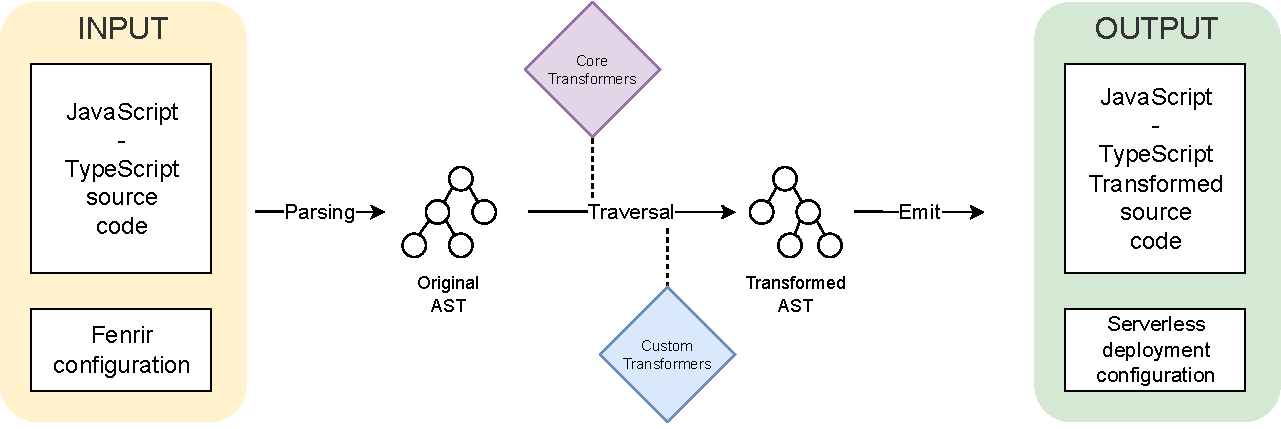
\includegraphics[width=\textwidth]{diagrams/pipeline}
  \caption{Transpiler pipeline.}
  \label{fig:pipeline}
\end{figure}

The transpilation pipeline, depicted in Figure \ref{fig:pipeline},
starts with the parsing of the input source code, which produces AST nodes with their related
annotations. Then, each annotation induces the application of its related
transformation step, whose output is fed into the next transformer, if any.
During the transformation steps, \f{} reports possible errors by gracefully
stopping the compilation process and indicating the offending instructions. Once
the transformations have taken place without any errors, the output code is saved
and the related metadata is also appended to a
\verb|serverless.yml| file which specifies function deployment
properties (e.g., the address to invoke a given function).

It is important to notice that \f{} does not lock developers in managing their
functions only through its tools, instead, its primary objective is to facilitate
the incremental adoption of the serverless paradigm.

\subsection{Brief example: Monolith to Serverless conversion}
\label{sec:example}

In Listing~\ref{lst:source}, we show an example of a monolithic codebase with a
pair of illustrative functions. One function, called \verb|processOrder|,
retrieves orders (e.g., via a database query). The other function, called
\verb|generateReport|, produces reports based on the retrieved orders. Since
we want the \verb|processOrder| function to be invocable from clients, we
annotate it as \annotation{\$Fixed}, and we specify its HTTP endpoint and method
with the \annotation{\$HttpApi} annotation. The \verb|generateReport| function
is instead a backend one, which we want to run at pre-established intervals: to
obtain this behavior, we use the \annotation{\$Scheduled} annotation to specify
that it shall be run every two hours.
All these annotations are explored in detail in \cref{sec:annotations}.
Using \f{}, we translate the code of Listing~\ref{lst:source} into the
serverless codebase of Listings~\ref{lst:processOrder}--~\ref{lst:yaml}.

\begin{lstlisting}[language=javascript, caption={Source Code.}, label=lst:source]
/**
 * $\dollar$Fixed
 * $\dollar$HttpApi(method: "GET", path: "/orders/report")
 */
export async function processOrder(orderId) {
  // ... processing logic ...
  console.log(`Processing order $\dollar${orderId}`)
  return order
}
/** $\dollar$Scheduled(rate: "2 hours") */
export async function generateReport() {
  // get the processed data and generate report
  console.log("Generating report")
}
\end{lstlisting}

\begin{lstlisting}[language=javascript, caption={Generated Code.}, label=lst:processOrder]
export async function processOrder(event) {
  const orderId = event.orderId
  // ... processing logic ...
  console.log(`Processing order $\dollar${orderId}`)
  return {
    statusCode: 200,
    body: JSON.stringify(order),
  }
}
// The implementation of `generateReport`
// is omitted as it remains unchanged.
\end{lstlisting}

\begin{minipage}{\textwidth}
\begin{minipage}[t]{.5\textwidth}
\begin{lstlisting}[language=yaml]
processOrder:
  handler: output.processOrder 
  events:
    - httpApi: 
      method: GET
      path: /orders/report
\end{lstlisting}
\end{minipage}
\begin{minipage}[t]{.5\textwidth}
\begin{lstlisting}[language=yaml,firstnumber=last]
generateReport:
  handler: output.generateReport
  events:
    - schedule:
        rate: 2 hours
\end{lstlisting}
\end{minipage}
\captionof{lstlisting}{\label{lst:yaml}Generated deployment configuration.}
\end{minipage}

The generated code includes both the \verb|processOrder| and \verb|generateReport| functions ready to
be deployed on the serverless platform. In particular, notice that the input of
\verb|processOrder| changed to match the expected signature for functions of
the serverless platform, i.e., an \verb|event| that carries, among other
content, the invocation parameters of the function, which are automatically
assigned to local counterparts at the beginning of the function body.
Complementarily, we also find the return value changed to match the shape of the
response expected by the platform---at lines 5--8 of
Listing~\ref{lst:processOrder}, we create a JSON object with a status code and a
body that contains a serialized version of the value held by the variable
\verb|order|, which holds the value returned by the function in the source
codebase.
The other notable element in the YAML code found in
Listing~\ref{lst:yaml}, which contains the information that the serverless
platform needs to deploy the two functions, e.g., the type of invocation for the
\verb|processOrder| function (HTTP) and its invocation address and the call
schedule of the \verb|generateReport| function.

This brief example introduces features that will be thoroughly described,
but it does not contain any real logic.
A non-trivial example, named \textit{Hati}\footnote{In Norse mythology, Fenrir has two sons, Hati and Sköll.},
is present in the \f{} public repository, yet, it is omitted from this thesis due to its size.

\textit{Hati} converts a monolithic email message analysis program,
into an event-driven serverless pipeline where each function
has the same core logic as the monolithic counterpart, but they are manipulated to have
all the benefits offered by the serverless paradigm.

\begin{figure}[H]
  \centering
  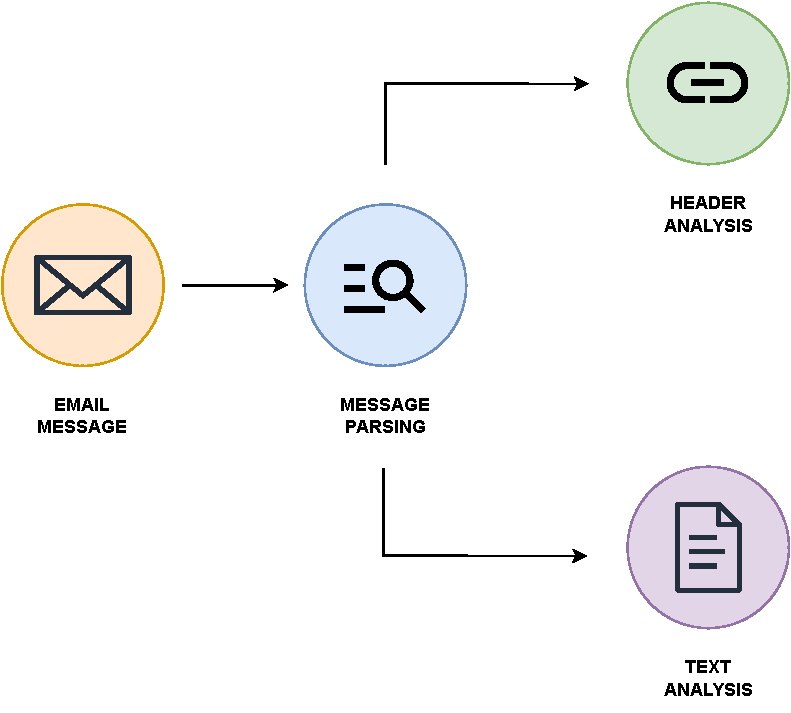
\includegraphics[width=0.7\textwidth]{diagrams/hati}
  \caption{\textit{Hati}'s pipeline.}
  \label{fig:hati}
\end{figure}

% \section{Detailed review}

% This section explains each step of the pipeline, defines annotations precisely and shows how to create new ones.

\section{Parsing}

\f{} requires a configuration file that must be named \verb|fenrir.config.json| to understand where to operate:

\begin{lstlisting}[language=json, caption={\f{} configuration}]
{
  "files": ["input/source.ts"],
  "serverlessConfigPath": "input/serverless.yml",
  "outputDirectory": "output",
  "annotations": {
    "CustomAnnotation": "annotations/custom-annotation.ts"
  }
}
\end{lstlisting}

The \verb|files| field accepts an array of filenames or a directory,
and it is used to represent which files will be parsed by the transpiler.

The \verb|serverlessConfigPath| field points at the input \textit{SLS} configuration
that must contain some mandatory input metadata, such as the region which the functions will be deployed on.

The \verb|outputDirectory| field indicates where the emitted files will be placed.

The \verb|annotations| field locates custom annotations as it takes an object
where the keys represent the new names and the values refer to their associated implementations.

\paragraph{\textbf{Fenrir's CLI}}
After creating the configuration, \f{} can be started through its CLI tool
by optionally passing as a flag the directory in which it is contained.
\begin{lstlisting}[language=bash, style=bashstyle]
# defaults to the current directory (.) for its file lookup...
> fenrir
# ...or uses a custom path
> fenrir -g input-directory
\end{lstlisting}
Furthermore, the CLI offers the \verb|init| sub-command to ease the setup needed for the entire pipeline
by generating the necessary boilerplate and configuration files.

\subsubsection{AST Traversal}

Through the \textit{TypeScript} compiler API, each sources' AST is traversed
by a visitor function which collects some data (e.g., dependencies imports) and examines
certain types of node in order to process annotations, namely \textit{exported function declarations}.
Lookups are restricted only to this syntactic category for two reasons:
\begin{itemize}
  \item \verb|export| ensures the functions are public and ready to be deployed.
  \item \verb|function declarations| minimize the code needed to control the AST.
    Considering that \textit{JavaScript} provides three distinct ways of declaring a function,
    accommodating all of these variations would inevitably result in a threefold expansion of the manipulation code.
    Moreover, function declarations are the idiomatic technique to write top-level functions.
\end{itemize}

\begin{lstlisting}[language=javascript, caption={Examples of processed or skipped nodes.}]
// Skipped
const a = 2;
// Skipped
for (const b of [1, 2, 3]) {}
// Processed
export function foo() {}
// Skipped
export const fiz = () => {}
// Skipped
export const bar = function() {}
\end{lstlisting}

The processed functions have their annotations examined, and
their bodies are visited to handle AST transformations.

\section{Annotations}
\label{sec:annotations}

Annotations are syntactical units, or keywords, enclosed within JSDoc comments,
each associated with their respective transformer.
They can be expressed using a BNF-like syntax:
\begin{equation*}
\begin{aligned}
    \text{Annotation} & ::= "\$" \langle \text{Name} \rangle [ "(" \langle \text{Parameters} \rangle ")" ] \\
    \text{Name} & ::= [\text{a-zA-Z0-9\_}]+ \\
    \text{Parameters} & ::= \langle \text{TypeScriptObject} \rangle \\
    \text{TypeScriptObject} & ::= \dots \\
\end{aligned}
\end{equation*}
This representation does not intend to provide a formal and complete definition of the syntax of annotations.
Nevertheless, it serves to offer a general intuition of how they can be written within the code.
\begin{lstlisting}[language=javascript, caption={Generic examples of annotation.}, label={lst:annotations-examples}]
/** $\dollar$Foo */

/** $\dollar$Bar(param: "first") */

/** $\dollar$Fiz(first: true, second: [1, 2, 3], third: (a, b) => a + b) */

/**
 * Annotations enrich docs...
 * $\dollar$Foo
 * ...and can even be multiline.
 * $\dollar$Bar(
 *    param: "fiz"
 * )
 *
 * all these explanatory texts are not 
 * harmful, as they are simply ignored.
 */
\end{lstlisting}

Annotations are designed to avoid cluttering \textit{JavaScript} code with new syntax,
as they can only be written inside JSDoc comments.
Thus, they serve a dual-purpose, they provide the functionality needed by \f{},
and they also serve as supplementary documentation for the codebase.

Listing \ref{lst:annotations-examples} provides a valuable insight on how annotations
may be parameterized to modify transformers' functionality.
In fact, arguments undergo parsing as a \textit{TypeScript} object literal,
hence, they are as powerful as regular objects~\cite{mdn_objects}
meaning that even complex structures (arrays, functions, etc...) can be used
during the compilation step to enrich transformations.

Another crucial feature of annotations is their composability,
as multiple annotations can be written within the same JSDoc,
essentially defining dedicated compilation pipelines by passing the output
of a transformation as input for the subsequent ones:
to facilitate this process, each source file may be visited multiple times.

\subsection{Core Annotations}

\f{} offers four core annotations whose transformers can handle code manipulation,
deployment metadata or a combination of both functionalities:
by pipelining annotations, we can effectively utilize the strengths of different approaches.

\begin{table}[htbp]
    \centering
    \caption{Core annotations}
    \begin{tabular}{llcc}
        \toprule
        \textbf{Name} & \textbf{Code} & \textbf{Metadata} \\
        \midrule
        \$Fixed & Yes & Yes \\
        \$TrackMetrics & Yes & No \\
        \$HttpApi & No & Yes \\
        \$Scheduled & No & Yes \\
        \bottomrule
    \end{tabular}
\end{table}

\subsubsection{\$Fixed}
\annotation{\$Fixed(memorySize?: number, timeout?: number, ...)}
converts monolithic functions into \textit{fixed}-size serverless functions,
whose resources are statically determined and remain constant regardless of the workload or input size.
To achieve this conversion, code is handled as follows:
\begin{itemize}
  \item The monolithic functions' parameters are mapped to a single \verb|event|
    parameter in order to adhere to \textit{AWS Lambda} serverless functions' signature.
  \item The monolithic functions' return statements change to match
    the shape of the response expected by the platform,
    by creating an object with a status code (\verb|200|)
    and a body that contains a serialized version of the initially returned value.
  \item Early return statements and throw statements are modified similarly,
    but the status code represents a client error (\verb|400|).
\end{itemize}

\annotation{\$Fixed} has no mandatory parameters, however, all the specified arguments will be
passed as metadata for the function deployment.

% ----------------------------------------------------------
% FIXED EXAMPLE
% ----------------------------------------------------------
\begin{lstlisting}[language=javascript, caption={Input code for \annotation{$\dollar$Fixed}}]
/** $\dollar$Fixed(timeout: 10) */
export async function foo(id) {
  if (!isValid(id)) {
    throw new Error('Something went wrong')
  }

  const data = await query()

  return data
}
\end{lstlisting}


\begin{lstlisting}[language=javascript, caption={Output code from \annotation{$\dollar$Fixed}}]
/** $\dollar$Fixed(timeout: 10) */
export async function foo(event) {
  const id = event.id

  if (!isValid(id)) {
    return {
      statusCode: 400,
      body: JSON.stringify({
        error: "'Something went wrong'",
      }),
    }
  }

  const data = await query()

  return {
    statusCode: 200,
    body: JSON.stringify(data),
  }
}
\end{lstlisting}

\begin{lstlisting}[language=yaml, caption={Generated Metadata through \annotation{$\dollar$Fixed}}]
functions:
  foo:
    handler: output/source.foo
  timeout: 10 # default is 6 seconds
\end{lstlisting}
% ----------------------------------------------------------
% FIXED EXAMPLE
% ----------------------------------------------------------

\subsubsection{\$TrackMetrics}
\annotation{\$TrackMetrics(namespace: string, metricName: string, metricValue?: ts.Expression)}
generates code that monitors and logs the functions’ resource usage
by also importing the necessary dependencies, i.e., for \textit{AWS Lambda}
it uses and injects the \textit{CloudWatch} dependency.
These are the required properties:
\begin{itemize}
  \item The function declaration must be \verb|async|.
    Preceding this annotation with \annotation{\$Fixed} makes it automatically \verb|async|.
  \item \verb|namespace| and \verb|metricName| are mandatory strings.
    The former represents the namespace instantiated on the cloud through \textit{AWS}.
  \item The third parameter, if present, must be the same as one of the variables' identifiers.
\end{itemize}

We complete the explanation with an example:
% ----------------------------------------------------------
% TRACK EXAMPLE
% ----------------------------------------------------------
\begin{lstlisting}[language=javascript, caption={Input code for \annotation{$\dollar$TrackMetrics}}]
import { query } from './local'

/**
 * $\dollar$TrackMetrics(namespace: 'shop', metricName: 'sell', metricValue: size)
 */
export async function processOrder(id) {
  const order = await query(id)
  const size = order.size
  // ...more logic...
  return size
}
\end{lstlisting}


\begin{lstlisting}[language=javascript, caption={Output code from \annotation{$\dollar$TrackMetrics}}, label={lst:out-track}]
import { query } from './local'
import { CloudWatch } from 'aws-sdk'

/**
 * $\dollar$TrackMetrics(namespace: 'shop', metricName: 'sell', metricValue: size)
 */
export async function processOrder(id) {
  const order = await query(id)
  const size = order.size
  await new CloudWatch()
    .putMetricData({
      Namespace: 'shop',
      MetricData: [
        {
          MetricName: 'sell',
          Timestamp: new Date(),
          Value: size,
        },
      ],
    })
    .promise()
  // ...more logic...
  return size
}
\end{lstlisting}
% ----------------------------------------------------------
% TRACK EXAMPLE
% ----------------------------------------------------------

Listing \ref{lst:out-track} shows the generated boilerplate to enable logs inside the function,
and an additional import statement is included at the top of the file to address its previous absence.
\annotation{\$TrackMetrics} puts the code in a context-aware manner,
placing it after the variable declared as \verb|metricValue|.

Supposing a typographical error was written instead of \verb|size|, the following error message would appear:
\begin{lstlisting}[language=console]
'$\dollar$TrackMetrics' can only receive an identifier as
a value for the 'metricValue' parameter like
'id' | 'order' | 'size'
in function 'processOrder' defined here:
--> input/source.ts:6
\end{lstlisting}

\subsubsection{\$HttpApi}
\annotation{\$HttpApi(method: string, path: string, ...)}
generates the metadata needed to make the function available as an HTTP endpoint.
\begin{itemize}
  \item The \verb|method| parameter represents the desired HTTP method (\verb|GET|, \verb|POST|, etc...).
  \item The \verb|path| parameter represents the URL path where the function will be available.
  \item The optional parameters are meant to customize the behavior of the HTTP endpoint further,
     for example, by setting up Cross-Origin Resource Sharing (CORS) headers.
\end{itemize}
% ----------------------------------------------------------
% Http EXAMPLE
% ----------------------------------------------------------
\begin{multicols}{2}[\columnsep=1cm]
\begin{lstlisting}[language=javascript]
/**
 * $\dollar$HttpApi(method: "POST", path: "/users/create")
 * $\dollar$HttpApi(method: "PUT", path: "/users/update")
 */
export function foo() {}
\end{lstlisting}

\columnbreak

\begin{lstlisting}[language=yaml]
foo:
  handler: output/source.foo
  events:
    - httpApi:
        method: POST
        path: /users/create
    - httpApi:
        method: PUT
        path: /users/update
\end{lstlisting}
\end{multicols}
% ----------------------------------------------------------
% Http EXAMPLE
% ----------------------------------------------------------

\subsubsection{\$Scheduled}
\annotation{\$Scheduled(rate: string, ...)}
generates the metadata needed to make the function run at specific dates or periodic intervals.
\begin{itemize}
  \item The \verb|rate| parameter is a rate or cron expression
    which schedules when the function should be triggered.
  \item The optional parameters are meant to customize the behavior of the scheduled event further,
     for example, by specifying multiple schedule expressions and giving it a description.
\end{itemize}
% ----------------------------------------------------------
% Scheduled EXAMPLE
% ----------------------------------------------------------
\begin{multicols}{2}[\columnsep=2cm]
\begin{lstlisting}[language=javascript]
/**
 * $\dollar$Scheduled(rate: "rate(2 hours)")
 */
export function foo() {}
\end{lstlisting}
\columnbreak

\begin{lstlisting}[language=yaml]
foo:
  handler: output/source.foo
  events:
    - schedule:
        rate: rate(2 hours)
\end{lstlisting}
\end{multicols}
% ----------------------------------------------------------
% Scheduled EXAMPLE
% ----------------------------------------------------------

\subsection{Custom Annotations}

\f{} is not bound to its core annotations, as it endorses the creation of new ones
to fit custom requirements and usages.

In order to inform \f{} of the new annotation name and its transformer implementation,
the configuration file (i.e., \verb|fernrir.config.json|) must be updated:
\begin{lstlisting}[language=json]
{
  ...
  "annotations": {
    "IoT": "annotations/iot-impl.ts"
  }
}
\end{lstlisting}

\f{} encourages strict type-safety by offering a type definition for custom transformers:
\begin{lstlisting}[language=javascript, caption={Custom transformer for a new \annotation{$\dollar$IoT} annotation.}, label={lst:custom-transformer}]
// in 'annotations/iot-impl.ts'
import type { CustomTransformer } from 'fenrir-core'

type IotTransfomer = CustomTransformer<'IoT', { sql: string }>

const transformer: IotTransfomer = (
  node,
  context,
  annotation
) => {
  // ...implementation...
}

// custom transformers must be exported as `default`
export default transformer
\end{lstlisting}

Analyzing custom transformers' signature also provides insights on how
core annotations are implemented, since their definitions are almost identical.

The \verb|node| argument represents the function declaration in the AST which was marked with the annotation.
It contains all the relevant information associated with this type of AST node,
including the function's body, name, parameters, and other relevant details.

The \verb|context| argument represents the \textit{TypeScript} transformation context,
which is a very powerful object containing:
\begin{itemize}
  \item Methods for source code manipulations, such as\\\verb|context.factory.updateIfStatement()|.
  \item The typechecker, which is an essential module integrated in \textit{TypeScript}, useful for working with symbols:
    it has access to every type of each node and details about the project dependencies.
  \item Miscellaneous methods to handle lexical environments and compiler options.
  \item \f{} utilities that facilitate the development of transformers and of metadata handling.
\end{itemize}

The \verb|annotation| argument is an object containing the annotation name
and a record of all the arguments passed to it.
Its type definition is inferred from the previously established \verb|CustomTransformer| schema.

A transformer's return type can be omitted as it is inferred, however,
if it is manifested to provide a stricter signature, it is restricted to this subset:
\begin{lstlisting}[language=javascript, numbers=none]
type TransformerReturnType =
  | ts.SourceFile
  | ts.FunctionDeclaration
  | undefined
  | void
\end{lstlisting}
Hence, transformers may perform three types of tasks:
modifying the entire source file, which is useful for updating import declarations or other AST nodes,
altering the function itself,
or solely modifying the metadata without changing the source code.

\section{Emit}

The last step of \f{}'s pipeline involves emitting the transformed files and metadata.
Files are ejected in a single output folder,
with the default name being \textit{functions}: it is important to give it an insightful name,
since, users are encouraged to review and potentially modify the emitted code
if they aren't satisfied with the transformations.

The transformed code may not look as the input code, as it is formatted
through an opinionated set of conventions which imposes properties like
the usage of semicolons or the number of spaces:
in order to make it adhere to personal formatting preferences,
users should use popular tools such as \textit{ESLint} and \textit{Prettier}.

Generated metadata is appended to a \verb|serverless.yml| placed at the project root,
and through the \textit{SLS} CLI it may be deployed to the serverless platform.

\subsection{Error handling}

\f{} tries to provide as many informations as it can when it meets errors.

Configuration mistakes cause the program to panic, for example:
\begin{lstlisting}[language=console]
Since you are providing a list of files, a `serverless.yml` must
be provided to the transpiler to generate the needed metadata.
\end{lstlisting}

Annotations syntax errors provide another set of logs:
\begin{lstlisting}[language=console]
$\dollar$Schdle
 ^^^^^^
 Unknown annotation name

$\dollar$Scheduled(
          ^
          Invalid bracket

$\dollar$Fixed(foo: )
      ^^^^^^^
      Invalid syntax for annotation parameters
\end{lstlisting}

Transformers can also emit specific errors only related to their domain, such as:
\begin{lstlisting}[language=console]
'$\dollar$HttpApi' must receive both 'method' and 'path' as parameters
in function 'foo' defined here:
--> input/source.ts:6
\end{lstlisting}

\chapter{Conclusions}
\label{chap:conclusion}

After a brief introduction, we discussed all the necessary knowledge needed
to understand this thesis in \cref{chap:background}, and finally we inspected
how \f{} works by thoroughly examining its inner components in \cref{chap:implementation}.

The most important concept to recall about this framework is its goal,
and how it tries to achieve it.
\f{} wants to enhance the serverless model through its meta-programming
features. In fact, its core annotations operate very differently from each other,
as they are related to distinct domains, but they still can be combined
to enrich the development experience.
Thus, \f{}'s users are not only inheriting all the
benefits offered by serverless architectures,
but they are also accessing all its powerful code
transformations that can save precious development time.

\f{} was also designed to help migrate existing
monolithic codebases into serverless ones through an incremental approach,
meaning that, users do not need to convert their entire project, but they
can partially adopt this new computing paradigm by iteratively rewriting features.
Additionally, it is crucial to comprehend that the code
emitted by \f{} is not set in stone, instead, it can be actively modified
and even used as a starting point for the codebase.
\f{} should be viewed as a co-pilot rather than a fully comprehensive tool to write serverless functions.

\f{}'s most notable limitation is the lack of more core annotations,
which stems from the substantial time investment required
to establish the framework's foundations, reflect on valuable transformers and write their implementation.
Still, users are encouraged to create their custom annotations
tailored to address their specific use cases, which can include scenarios
that cannot be foreseen by \f{} due to their unique nature.

Another important decision to discuss is our rationale behind selecting \textit{TypeScript}.
Many other programming languages offer meta-programming compile-time capabilities,
like \textit{Rust} macros, \textit{C++} templates or \textit{Zig} comptime:
such systems are far superior to our annotations, yet,
these low-level languages are not suitable for the high-level programming
that the serverless functions are supposed to entail, in fact most of these languages
do not have the runtime support from any major platform provider.
Moreover, even high-level languages with similar compile-time features like \textit{Scala}
demand to be monitored with caution, because of their heavy
runtime (i.e., \textit{JVM} for \textit{Scala}) initialization spin-ups
that may cause expensive cold starts.

\textit{TypeScript}, enriched with our annotations, perfectly fits
the serverless model as it runs, after its strict static type checks,
on \textit{Node.js}, which is a well-suited lightweight environment
designed to handle distributed services as discussed in \cref{sec:node}.

\section{Comparison with previous studies}

One of the features offered by \f{} is the fact that it can port
an existing monolith to a serverless platform as shown in \cref{sec:example}.
This process, named ``FaaSification'', has captured the attention of researchers
who have explored and presented various solutions to this challenge.

The first attempts were developed for \textit{Python} and \textit{Java} monoliths,
with the tools being named respectively \textit{Lambada} \cite{lambada} and \textit{Termite} \cite{termite}.
They are fairly limited as their emitted code cannot correctly process inputs,
and they do not support the use of global variables within the serverless functions.

Instead, let us focus on the technologies built around \textit{JavaScript}:

\paragraph{\textbf{Node2Faas} \cite{node2faas}}
It was the first \textit{JavaScript} ``faasifier'':
it converts methods of the \textit{Node.js} monolith into serverless
functions and replaces their bodies with an API call to the target FaaS system.
This tool has many weaknesses: most notably it cannot resolve neither code
nor package dependencies, which is a considerable constraint since many
cloud functions work by using third-party services.

\paragraph{\textbf{DAF} and \textbf{M2FaaS} \cite{daf, m2faas}}
They were built by the same team of researchers, the latter, \textit{M2FaaS},
represents an improved iteration of the former.
They introduce a concept similar to our annotations, through which users
can mark arbitrary parts of their code with the dependencies needed to be deployed.
The outcome is a serverless monolithic application hybrid. 
However, due to technical limitations, the development effort to write their marking constructs
is remarkable as users are compelled to write configuration details inside their business logic.

\paragraph{\textbf{FaaSFusion} \cite{faasfusion}}
This is the closest work to \f{}.
\textit{FaaSFusion}'s users also mark their functions with annotations
and some associated code transformations occur.
This framework brings infrastructure-as-code concepts into the function source,
but this approach has evident shortcomings since it heavily relies on heuristics for its foundations.
For example, it offers an annotation named \annotation{@Warmup} which
injects an algorithm to avoid cold starts by periodically pinging the function
through a \textit{CloudWatch} event:
however, platform providers have suggested avoiding these so-called ``warmers'',
because they are mostly ineffective, break serverless principles, and can increase costs very quickly.

The main obstacle that these tools do not overcome is that they are
not designed to handle codebases beyond the trivial examples
which they present to support their cases.
In comparison, \f{} is very powerful, and its scope is broader
as it represents more than a simple ``faasifier''.

\section{Future directions}

We believe \f{} could be improved further by expanding its features
or by building tools built around it.
We close this thesis by listing a few of the enhancements \f{} could receive.

\subsection{More annotations}

\f{} should have more core annotations.
Also, while the existing annotations currently don't exhibit conflicts with each other,
it's prudent to anticipate potential conflicts that could arise when new annotations are introduced:
consequently, incorporating new constraints becomes essential to prevent such
conflicts and ensure the smooth coexistence of annotations within the framework.

\f{} should add support for marking not just top-level functions, but also other AST nodes.
This feature would enrich the framework further, as users would have more freedom
to change how transformations happen. These new annotations may be inside the function itself,
marking nodes inline, or even at the source level. Additionally, they may be related to a particular annotation,
thus, creating sets of domain-specific annotations.
For example, \annotation{\$Fixed}, whose objective is related to ``faasification'',
could have \textit{children} annotations that would issue a warning if used under other top-level annotations.
\begin{lstlisting}[language=javascript]
/** $\dollar$Fixed */
export async function foo() {
  const data = await query()
  // new inner annotation, which changes parts of the emitted code
  /** $\dollar$StatusCode(code: 201) */
  return data
}
\end{lstlisting}

\subsection{Formalization}

Many parts of this framework should be formalized, similarly to the work conducted by Kallas et al. \cite{formalization},
as this would give solid foundations to \f{}:

\begin{itemize}
  \item Annotation syntax and semantics, including defining
    the structure of annotations, allowed parameters, and their meanings,
    because we only presented an preliminary insight in \cref{sec:annotations}.

  \item Composition semantics to spot potential conflicts between annotations.

  \item Transformations algorithms to ensure correctness, predictability,
    and consistency in the compilation process, given some notion of behavioral correspondence.
\end{itemize}

\subsection{Linter}

Linter.

Choral


% This ensures that the subsequent sections are being included as root
% items in the bookmark structure of your PDF reader.
\bookmarksetup{startatroot}
\backmatter
  \printbibliography
  \cleardoublepage % start the page at right
\phantomsection
\addcontentsline{toc}{chapter}{Ringraziamenti}
\chapter*{Ringraziamenti}
\pagestyle{empty}
\thispagestyle{empty}
\markboth{Ringraziamenti}{Ringraziamenti}

Lorem ipsum dolor sit amet, officia excepteur ex fugiat reprehenderit enim labore culpa sint ad nisi Lorem pariatur mollit ex esse exercitation amet. Nisi anim cupidatat excepteur officia. Reprehenderit nostrud nostrud ipsum Lorem est aliquip amet voluptate voluptate dolor minim nulla est proident. Nostrud officia pariatur ut officia. Sit irure elit esse ea nulla sunt ex occaecat reprehenderit commodo officia dolor Lorem duis laboris cupidatat officia voluptate. Culpa proident adipisicing id nulla nisi laboris ex in Lorem sunt duis officia eiusmod. Aliqua reprehenderit commodo ex non excepteur duis sunt velit enim. Voluptate laboris sint cupidatat ullamco ut ea consectetur et est culpa et culpa duis.

\clearpage


\end{document}
